\chapter{Introduction and Background}


\section {A brief overview}


\section{Neutron transport}
Neutron transport is required when modeling nuclear reactor physics as it describes where and how neutrons produce fission reactions which in turn generate heat in the fuel rods \cite{Duderstadt1971NuclearAnalysis}. Modeling this is necessary for both the analytical design and safety analysis of a reactor. Assuming no neutrons are being produced by fission, the neutron transport equation (NTE) takes the form of an intergro-partial differential Boltzmann-type equation with seven independent variables:
\begin{multline}
    \label{eq:fullNTE}
    \frac{1}{v(E)}\frac{\partial \psi(\boldsymbol{r}, E, \boldsymbol{\hat{\Omega}},t)}{\partial t} + \boldsymbol{\hat{\Omega}} \cdot \nabla \psi(\boldsymbol{r}, E, \boldsymbol{\hat{\Omega}},t) + \Sigma_t(r, E, t) \psi(\boldsymbol{r}, E, \boldsymbol{\hat{\Omega}},t) = \\
    \int_{4\pi}\int_{0}^{\infty}\Sigma_s(\boldsymbol{r}, E'\rightarrow E, \boldsymbol{\hat{\Omega}'} \rightarrow \boldsymbol{\hat{\Omega}}, t)
    \psi(\boldsymbol{r}, E, \boldsymbol{\hat{\Omega}},t) dE' d\boldsymbol{\hat{\Omega}'} +
    s(\boldsymbol{r}, E, \boldsymbol{\hat{\Omega}},t) \;,
\end{multline}
where $\psi$ is the angular flux, $v$ is the velocity of the particles, $\Sigma_t$ is the macroscopic total material cross section, $\Sigma_s$ is the macroscopic scattering cross section, $\boldsymbol{r}$ is the location of the particle in three-dimensional space, $\boldsymbol{\hat{\Omega}}$ is the direction of travel in three-dimensional space, $s$ is the source of new particles being produced, $t$ is the time, and $E$ is the energy of the particles for $\boldsymbol{r} \in V$, $\boldsymbol{\hat{\Omega}} \in 4\pi$, $0<E<\infty$, and $0<t$. We also prescribe the initial condition
\begin{equation}
    \psi(\boldsymbol{r}, E, \boldsymbol{\hat{\Omega}},0) = \psi_{initial}(\boldsymbol{r}, E, \boldsymbol{\hat{\Omega}})
\end{equation}
and the boundary condition
\begin{equation}
    \psi(\boldsymbol{r}, E, \boldsymbol{\hat{\Omega}},t) = \psi_{bound}(\boldsymbol{r}, E, \boldsymbol{\hat{\Omega}},t) \text{ for } \boldsymbol{r} \in \partial V \text{ and } \boldsymbol{\hat{\Omega}} \cdot \boldsymbol{n} < 0 \;.
\end{equation}

This equation is commonly solved using both deterministic and Monte Carlo scheme


\section {Deterministic Methods}
When solving the neutron transport equation with deterministic scheme a list of assumptions can be utilized to simplify \refeq{eq:fullNTE} into something tractable. Isotropic scattering, slab geometry, S$_N$ approximation in angle, isotropic sources, the multi-group assumption in 
\begin{multline}
    \label{eq:sn_nte}
    \frac{1}{v_g} \frac{\partial \psi_{m,g}(x,t)}{\partial t} + \mu_m \frac{\partial \psi_{m,g}(x,t)}{\partial x} + \Sigma_g(x) \psi_{m,g}(x,t)  \\
     = \frac{1}{2} \left( \sum\limits_{g' = 0}^G \Sigma_{s, g'\to g}(x) \sum\limits_{n=1}^N w_n \psi_{n, g'}(x,t) + Q_g(x,t) \right) \;, \\
    \qquad g=1 \ldots G \;, \qquad m=1 \ldots N \;, \qquad t > 0 \;, \qquad x \in [0,X] \;,
\end{multline}
where $\psi$ is the angular flux, $t$ is time, $x$ is location, $v$ is velocity, $w_m$ is angular quadrature weight, $\mu_m$ is the angular quadrature ordinate, $m$ is the quadrature index, and $Q$ is the isotropic material source.
The initial and boundary conditions are prescribed angular flux distributions:
\begin{equation*}
    \psi_{m,g}(x,0) = \psi_{m,0}(x), \qquad m=1 \ldots N \;,
\end{equation*}
\begin{equation*}
    \psi_{m,g}(0,t) = \psi_{m,L}(t), \qquad \mu_m >0 \;,
\end{equation*}
\begin{equation*}
    \psi_{m,g}(X,t) = \psi_{m,R}(t), \qquad \mu_m <0 \;.
\end{equation*}

From here classes of discretization can be used to turn the continues functions of angular flux, source, material data, and differential operators into numerical approximations.

\subsection{Discretization Schemes}



\subsubsection{Space discritizations}
To treat the space discretization various classes of numerical approximation can be used.
Finite difference, finite element and finite volume shchemes are all often employed with the Dimond-differncing scheme 
In 1D many FEM schems can look like FVM
The important distintion is that finite volume schemes are conservitive menaing they enforce continuity for any solver perameter

% introduce simple corner balance and explain why we used that one



\subsubsection{Time discritization}
The transport equation requires some kind of iterative scheme to converge the linkage between scattering source and transport operators (this is discussed more in section \ref{sec:intro_itterative-scheme}).
Thus implicit schemes are normally used to time step as there is no added cost of the iteration.
Specifically, implicit (backward) Euler (O1) or Crank-Nicolson (O2) are the most often employed.
These two schemes are advantageous as they often act like a wrapper scheme around a steady state deterministic transport solver with few changes needed to implement.

% why are they disadvatnagious

Other schemes have been 

% introduce TDMB


\subsection{Source-Iteration}
\label{sec:intro_itterative-scheme}

The source iteration (SI) method is commonly used to do this, often accompanied by preconditioners or synthetic accelerators, where the contribution to the solution from the scattering source is allowed to lag, while the angular flux is solved in every ordinate via transport sweeps through the spatial domain~\citep{adams_subcell_1997}.
SI sweeps in Cartesian geometries are readily parallelized over the number of angles, as the source term is known from the previous iteration, allowing the angular flux in each ordinate to be computed independently. 
While any parallelization is a boon to performance, a scheme that is embarrassingly parallel over the dimension with the greatest number of degrees of freedom---space---may be advantageous.
In a single spatial dimension SI is \textit{annoying serial} in space and cannot be parallelized.

In higher spatial dimensions, many $S_N$ production codes that implement SI use some kind of wavefront marching parallel algorithm also known as a Kockh-Baker-Alcouff scheme \citep{KBA}.
This is also called "full parallel sweeps" (FPS) in literature.
In this scheme a sweep begins in a spatial location where all cell dependencies are known from boundary information (e.g. a corner).
From there on a hypothetical 2D grid, the two nearest neighbor cells are now able to be computed independently, the next step would be 4 cells.
This diagonally marching wavefront continues to march widening paralleling as many cells spatially as possible eventually saturating the number of work threads if the problem is large enough.
On CPUs this has been shown to be performant but this changing amount of work is not optimal on GPUs where 
KBA algorithms are also tricky to efficiently implement in domain decomposed where wave front propagation between boundaries can be tricky.
While this work is concerned with 1 spatial dimension when analyzing the state of the art it is important to consider that this is done.

This has proven successful in modern transport applications on CPUs 
(e.g., PARTISN, which implements the Koch--Baker--Alcouffe or KBA algorithm ). 
The state of the art in deterministic $S_N$ radiation transport is multi-group in energy distribution, diamond differencing first order space discretizations, backward euler time stepping, domain decomposition via parallel block jacobi, wave front marching schemes like KBA in higher spatial dimensions within a subdomain, and source iterations with diffusion synthetic acceleration and GMRES solvers. Some examples of production codes that implement this are Partisn, Ardra, Minerate, Capsaicin, Denovo, Silver Fir, etc.


\subsection{One Cell Inversion-Iteration}

% Intro to OCI and previous work including warsaw 

One Cell Inversions (OCI) (also called cell-wise parallel block Jacobi) is an alternative to SI where all angular fluxes in all ordinates within a cell are computed in a single linear algebra step. It assumes that the angular fluxes incident on the surfaces of the cell are known from a previous iteration.
OCI allows for parallelizing over the number of cells as each cell is solved independently of the others in a parallel block Jacobi scheme. Block

\cite{rosa_cellwise_2013} previously investigated OCI as a potentially superior iterative scheme over SI on vectorized architectures.
They supposed that because of the parallelism over the dominant domain, inherit data locality, ability to take advantage of LAPACK type libraries, highly floppy operations present in an OCI type algorithm, it might out-perform a SI based implementation in wall clock runtime.
The study was conducted on state of the art at the time RoadRunner super computer and took advantage of its 64 bit PowerXCell vectorized accelerator based.
While not specifically designed as a GPU, notably versions of the Cell Broadband Engine architecture would be used on the Sony Playstation 3 gaming console.
Rosa et. al. implemented OCI in a 2D, multi-group, steady state, code using first order diamond differencing to discretize space, a multi-group scheme in energy distribution, and parallel block Jacobi and Gauss-Sidle iterations.

The authors concluded that the acceleration seen per iteration in an OCI implementation was not enough to make up fo the decay in convergence rate that OCI incurs.
Because there is no communication of information between cells within an iteration, OCI can require more iterations to converge to a solution for some of problems. 
Specifically, as cellular optical thickness goes down, OCI's relative performance degrades.
Figure~\ref{fig:specrad} illustrates this behavior, showing the spectral radii of the two iteration schemes as a function of cell thickness (in mean free path) and the scattering ratio.
These values were computed numerically from an infinite medium problem (via reflecting boundaries) using steady-state calculations in $S_4$. 
Gauss Legendre quadrature was used in all presented explorations.
The smaller the spectral radius, the faster a method is converging.
The spectral radius for SI depends strongly on the scattering ratio, and for problems that are many mean free paths in size, it is nearly independent of cell optical thickness. 
The spectral radius of OCI decreases substantially as the optical thickness of the cells increases.

\begin{figure}[!htb]
    \centering
    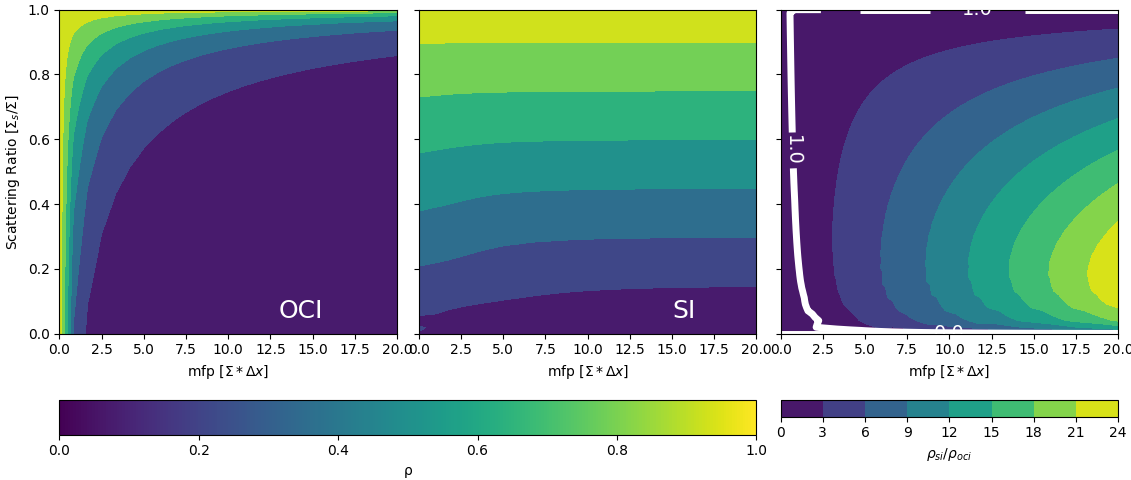
\includegraphics[width=\textwidth]{figures/spec_rad.png}
    \caption{Spectral radii ($\boldsymbol{\rho}$) of OCI (left) and SI (middle) and the ratio between the two (right), where $\boldsymbol{\Sigma}$ is the total cross section, $\boldsymbol{\Delta x}$ is the cell width, and $\boldsymbol{\Sigma_s}$ is the scattering cross section}
    \label{fig:specrad}
  \end{figure}

Rosa et. al. concluded by suggesting that future developments in GPGPU accelerators might overcome this hurtle.

Other investigations have explored OCI as an acceleration scheme for SI \citep{anistratov_iterative_2015, hoagland_hybrid_2021} and a solution to the Integral transport matrix method \citep{raffi2108pidotscom}.
Previous investigations of OCI have been limited to single order discretization schemes and steady state computations.

\subsection{Acceleration and Precondition}



\section {Monte Carlo methods}
Whereas deterministic numerical methods (e.g., forward Euler, Crank--Nicholson, Gaussian Quadrature) are applied to the governing integro-partial differential equations themselves, direct simulation Monte Carlo (or just Monte Carlo) is used to simulate the actual subatomic particles and how they interact with a given system \cite{CompMeth}.
Here known material composition and interaction rates of the particles at all speeds can be leveraged with pseudo-random numbers to individually simulate a particles life, aka history.

Take for example a shielding problem: where a beam of neutrons is impinging a slab of purely absorbing material.
Based off a cumulative probability distribution function we can supply a pseudo-random number between zero and one and the total material cross section (a known perimeter) to sample a distance to a collision.
We then compare the known width of the slab and the sampled distance to see if the particle made it through or was absorbed within. If this process is repeated a \textit{sufficient} number of times a statistically prevalent solution can be produced.

As the simulation grows more complex (e.g. scattering events, fission events, track length estimators, etc.) the computational work needed to simulate one neutron life time will go up.
Also as Monte Carlo methods converge at a rate of $O = \frac{1}{\log{n}}$ a massive number of particles may be required to gain a \textit{converged} solution.
All this is to say when using the Monte Carlo method on modern compute architectures it is often imperative to parallelize the algorithm.


\subsection{Portabilitiy Frameworks}
In recent years, many frameworks have appeared to solve portability issues, both between accelerator/HPC architectures and between different vendors of those architectures. 
Kokkos \cite{kokkos} is a portability framework developed by Lawrence Livermore National Laboratory.
When developing with Kokkos, a user declares and allocates memory, writes appropriate compute kernels (in Fortran, C++, or with limited operability in Python \cite{AlAwarETAL21PyKokkos}), and executes those functions with calls to the portability framework. 
When executed, the portability framework will make all architecture-specific API calls (i.e., \texttt{hipMemalloc}) independently of user-defined code.

%In recent years the Julia high level performance language has gained significant popularity and support for HPC architectures and accelerators.
%Julia acts as a light weight and approachable wrapper for the LLVM compiler framework, itself built for portability.
%Julia has support to run 

% how'd we get to python
Python is one of the most widely used programming languages, both generally and in academia.
It is dynamic, untyped, and supports a rich development environment for data processing with core scientific and numerical packages like NumPy \cite{van_der_walt_numpy_2011}.
For GPU support, tools like Cython, PyCUDA, and PyOpenCL \cite{kloeckner_pycuda_2012} can be used to compile and bind GPU functions---often written in \texttt{C++}---to Python code.
Often called Python-as-glue, these schemes can help in simplifying a code base that targets multiple accelerators but still require as many separate compute-kernel sources as hardware targets.
Different schemes have been implemented to alleviate source divergence for hardware targets when using Python-as-glue thus solving portability issue between hardware targets.
%divergent bakends code base per hardware target written in multiple languages.

Many tools have been developed to solve portability problems using Python.
One example is through using a domain-specific language (DSL) along with Python compiler tools to avoid needing a low-level language (e.g., FORTRAN, C).
A domain-specific language is designed specifically to alleviate development difficulties for a group of subject-area experts. 
It can even abstract hardware targets if it is defined with that goal.

PyFR, for example, is an open-source computational fluid dynamics solver that implements a DSL+Python structure \cite{witherden_pyfr_2014} to run on CPUs and Nvidia, Intel, and AMD GPUs. 
Portability is accomplished by writing the most compute-intensive kernels in a domain-specific language derived from the MAKO templating library. 
These kernels are called at run-time to compile the specialized numerical methods for a specific hardware target and bind it to Python. 
PyFR then uses Python tools to manage MPI calls, conduct I/O, pre- and post-process, compile, and manage the environment. 
Python, in this case, works as the glue language for the domain-specific one provided by MAKO. 
The overhead of this Python glue is less than 1\% in PyFR \cite{PyFR1p}.
While this development scheme does mean PyFR is written in two languages, only about 15\% of its structure is abstracted using the MAKO DSL.
As a result, PyFR has proven to be portable to various accelerators with compute kernels written in a single source. 
Withdren, et. al. \cite{pyfrPetascale} have discussed that this Python based scheme allows for rapid numerical methods development at deployment HPC scales. 
Using this tactic, they have successfully demonstrated PyFR's performance at the petascale \cite{pyfrPetascale}.

While this scheme works for PyFR and other codes like it, the nature of neutron transport means that employing a PyFR-like approach would result in a much higher percentage of a code-base implemented in the secondary DSL (whether MAKO, C++, or Fortran). 
In neutron transport, the compute kernel is the physics kernel.
A developer experimenting with and/or writing a novel numerical method will often be writing the most expensive compute kernels themselves. 
For example, when adding a tally to compute a new value, a developer could drastically alter the memory footprint of the computation. 
When adding a new event for a novel variance-reduction technique, they could introduce a critical divergence that will limit performance of that technique on GPUs. 
A DSL+Python scheme still requires developers to know two languages---one which is unique to the code at hand---and knowledge of the accelerator architecture to develop performant code.

Other modern codes have used completely Python-based solutions to create a portable, performant code base for both CPUs and GPUs.
Native Python is slow in terms of raw numerical performance.
However, packages like NumPy \cite{van_der_walt_numpy_2011} can do these operations significantly faster than the same algorithms in native Python for example if an algorithm depends on array-wise elemental operations.
Furthermore, multi-core CPU processing and targeting hardware accelerators can be provided by libraries that link into functions often written in Fortran or C (e.g., BLAS).

For example, Veros \cite{hafner_fast_2021}, a global ocean modeling code, implements this workflow:
numerical methods used to model the physics are deterministic, relying on array-type operations, like linear algebra. 
Veros uses the JAX library \cite{jax2018github} to compile NumPy-based operations into GPU compute kernels and Python-based MPI implementations for distributed memory parallelism. 
Hafner et al. \cite{hafner_fast_2021} show wall-clock speedup when implementing a JAX based development scheme, compared with the same algorithm traditionally implemented in a Fortran code.
They also show reasonable scaling across nodes up to 1000 MPI processes. 
JAX and NumPy allow Veros developers to implement performant code exclusively in pure Python, which can target both CPUs and GPUs.
Similar workflows that rely exclusively on commonly abstracted operations could be implemented by the CuPy \cite{cupy_learningsys2017} library, which binds into vendor-specific implementations of LAPACK/BLAS libraries.

Unfortunately, Monte Carlo kernels do not rely on these standard array-type operations.
Monte Carlo algorithms have very complex control flow that depends on the physics of the problem being modeled and decisions made by the user at run time. 
Even the most fundamental building blocks of a Monte Carlo code might have to be altered to implement a novel numerical method.

Other projects have addressed the need to write user defined compute kernels in a Python-based framework.
Sakras \cite{silvestri_sarkas_2022} is a molecular dynamics suite for plasma physics. 
It uses the Numba compiler to lower Python code with Numpy functions into LLVM, then just in time (JIT) compile those functions to a specific hardware \cite{lam_numba_2015}. 
The algorithms implemented in Sakras using Numba performed the same as when implemented purely in C.
While Sakaras only supports shared memory parallelism on a single-node, this development scheme could easily be paired with MPI to achieve distributed memory parallelism (as in the previous examples). 

Numba also compiles global and device functions for Nvidia GPUs from compute kernels defined in Python.
API calls are made through Numba on both the Python side (e.g., allocate and move data to and from the GPU) and within compiled device functions (e.g., to execute atomic operations).
When compiling to GPUs, Numba supports an even smaller subset of Python, losing most of the operability with NumPy functions.
If functions are defined using only that smallest subset, Numba can compile the same functions to CPUs or GPUs, or execute those functions purely in Python.
Numba data allocations on the GPU can be consumed and ingested by functions from CuPy if liner-algebra operations are required in conjunction with user-defined compute kernels.

%Numba has been shown to be slower then other high level portability frameworks for unoptimized matrix multiplication \cite{Godoy_2023}.
%Monte Carlo neutronic workflows are so memory bound that it's doubtful even significant changes to FLOP performance of a 

As any of these portability schemes would be novel when implemented in a Monte Carlo neutron transport application, we conducted an initial set of investigations to compare what we considered to be the most viable options at the time. 
We compared the same algorithm in various implementations using PyKokkos, PyCUDA/PyOpenCL, and Numba \cite{morgan2022}.
We found that all three methods produced similar runtimes for our workflows on CPUs and GPUs for a simple transient Monte Carlo neutron transport simulation.
Ultimately, we decided to use a Numba + mpi4py development scheme to build out a Monte Carlo neutron transport code for rapid numerical methods development, portable to various HPC architectures.

\section{GPU and GPU performance Anylisi}
% Kripkey performance published in gray literature
When analyzing performance on GPUs the roofline performance model is often used.
The roof is constructed by the communication or bandwidth (Bytes/S) and computation resources of a specific GPU for a specific numerical precision (floating operation points per second or FLOPS).
As algorithms at their most optimized become performance limited by either bandwidth or compute resources.
Thus when the performance of a given GPU device function is on the roofline it is the most optimized it could be.

Performance anylisys on GPUs of deterministic sweep codes is limited in the literature. 
That is espically the case when looking for roofline anylisys specifically.
Roofline models have previously been used to evalueate some miniapps in the Monte Carlo world \citep{tramm2021domain, tramm2022roofline}.

One place there is data on is a miniapp called cripky \citep{kunen_kripke_2015}.
Kripke is the publicly distributed version of Ardra that has performance data available.
Roofline anylisys of Kripke has been published for performance on an AMD MI200 GPUs \citep{wolfe2022roofline}. 
Specific k
We conject that this is due to the nonlinear work load a wavefront marching schemes incurred. 
As the wave moves through the problem space in a given ordinant the number of cells to be solved in parallel can change dramatically.
This kind of in kernel dynamic problem 
While our work is limited to a single spatial dimension thus avoiding anylisys of KBA algorithms this shows the state of the art in performance of deterministic code.


\label{ch-intro}